\documentclass[a4paper, 11pt]{article}
\usepackage{geometry}
\usepackage{indentfirst}
\usepackage{setspace}
\usepackage{amsmath}
\usepackage{graphicx}
\usepackage{wrapfig}
\usepackage{caption}
\usepackage{indentfirst}
\usepackage{amssymb}
\usepackage{float}

\graphicspath{ {./images/} }
\geometry{left=2.5cm, right=2.5cm, top=2.5cm, bottom=3cm}

\begin{document}
	% Upload all the source files and a report containing:
	% Answer to theoretical questions,
	% a brief description of the methods,
	% some comments to the results
	% all the outputs.
	
	\title{Exercise \# 1. Numerical methods for ODES. }
	\author{{\small Alexandre Rodrigues (2039952)}}
	\date{\today}
	
	\maketitle
	
	
	\section*{Methods}
		In this exercise I used the following methods to solve Ordinary Differential Equations:
		
		\subsection*{Simpson's Method}
		
		\subsection*{4-stage Runge-Kutta method (RK4)}
		
		\subsection*{Backwards Differentiation Formulas (BDF)}
		
		\subsection*{Crank Nicolson (CN)}
		
		
	
	
	\section*{Answers}
		% answer to theoretical questions
		\subsection*{Question 1}
		
		\begin{equation}
			y(t) = e^{-5t}
		\end{equation}
		
		\begin{figure}[H]
			\centering
			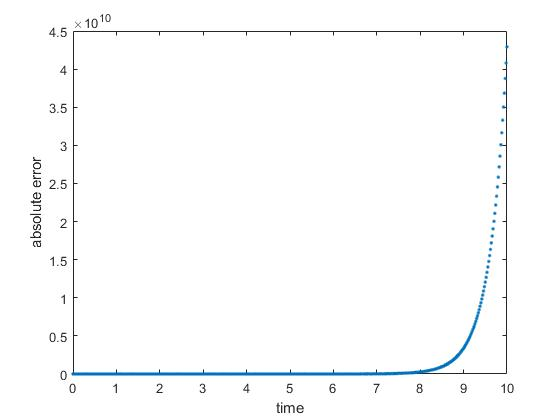
\includegraphics[width=\linewidth]{ex1_fe.jpg}
			\caption{Absolute error in function of time using Forward Euler method to compute y(1)}
			\label{fig:ex1_fe}
		\end{figure}
		
		The final error was $4.2916 \times 10^{10}$.
		
		\begin{figure}[H]
			\centering
			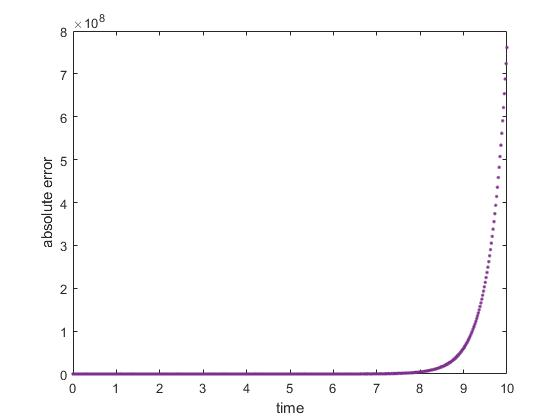
\includegraphics[width=\linewidth]{ex1_rk4.jpg}
			\caption{Absolute error in function of time using RK4 method to compute y(1)}
			\label{fig:ex1_rk4}
		\end{figure}
		
		The final error was $4.3146 \times 10^{10}$.
		
		The Simpson's method has an empty stability region as proved by: $\ldots$
		We can notice the difference in the initial conditions in our results.
		The FE calculation for y(2) is better then the RK4 calculation given the best final error.
		This is, although, not relevant because the difference is of about $ 0.5 \times 10^{-10} \% $.
		
		\subsection*{Question 2}
		
		The exact solution can be found as:
		\begin{equation}
			y(t) = \frac{1}{10t + 1}
		\end{equation}
		
		\begin{figure}[H]
			\centering
			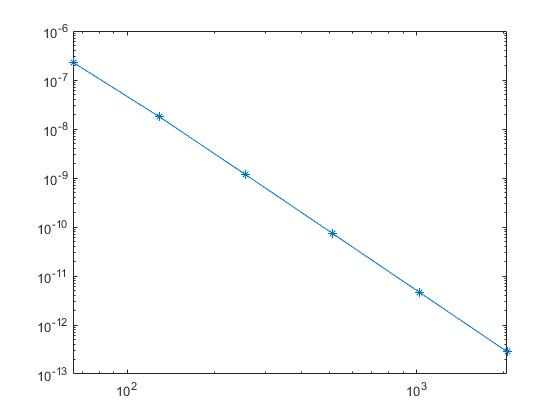
\includegraphics[width=\linewidth]{ex2.jpg}
			\caption{LogLog plot of the error as a function of the number of steps.}
			\label{fig:ex2}
		\end{figure}
		
		\begin{table}[H]
			\centering
			\begin{tabular}{c|c}
				\textbf{h}& \textbf{error}   \\ \hline
				$ 3.125000\times 10^{-2} $ & $ 2.291844\times 10^{-7} $ \\ \hline
				$ 1.562500\times 10^{-2} $ & $ 1.785763\times 10^{-8} $ \\ \hline
				$ 7.812500\times 10^{-3} $ & $ 1.160234\times 10^{-9} $ \\ \hline
				$ 3.906250\times 10^{-3} $ & $ 7.312862\times 10^{-11} $ \\ \hline
				$ 1.953125\times 10^{-3} $ & $ 4.579586\times 10^{-12} $ \\ \hline
				$ 9.765625\times 10^{-4} $ & $ 2.863750\times 10^{-13} $ \\ \hline
			\end{tabular}
		\end{table}
		
		The error reduces with the increase of the number of steps (decrease of $h$) as expected in theory.		
		
		\subsection*{Question 3}
		
		
		\subsection*{Question 4}
			\subsubsection*{Stability for RK4}
				As explained in the reference book \ref{book} on pages 19 and 20, we have the 4-th order Runge-Kutta method as:
				\begin{equation}
					y_{n+1} = (1 + \frac{1}{6}hk_1 + \frac{1}{3}hk_2 + \frac{1}{3}hk_3 + \frac{1}{6}hk_4)y_n
				\end{equation}
				, where
				\begin{align}
						k1 &= f(y_{n}) \\
						k2 &= f(y_{n} + \frac{h}{2} k_1) \\
						k3 &= f(y_{n} + \frac{h}{2} k_2) \\
						k4 &= f(y_{n} + h k_3)
					\end{align}
			
				Using $ \bar{h} = h\lambda $, one can simplify this equation to:
				\begin{equation}
					y_{n+1} = (1 + \bar{h} + \frac{1}{2}\bar{h}^2 + \frac{1}{6}\bar{h}^3 + \frac{1}{24}\bar{h}^4)y_n
				\end{equation}
				The relation of the current iteration value $y_n$ with the initial value $y_0$ is:
				\begin{equation}
					y_{n+1} = (1 + \bar{h} + \frac{1}{2}\bar{h}^2 + \frac{1}{6}\bar{h}^3 + \frac{1}{24}\bar{h}^4)^n y_o
				\end{equation}
			
				This implies the absolute stability region satisfies the following inequality:
				\begin{equation}
					|1 + \bar{h} + \frac{1}{2}\bar{h}^2 + \frac{1}{6}\bar{h}^3 + \frac{1}{24}\bar{h}^4| < 1 
				\end{equation}
				Assuming $h$ as a real number we have the following stability region:
				\begin{equation}
					-2.78529 < \bar{h} < 0
				\end{equation}
				
				This can be extended to a system of ODEs by using the largest modulus eigenvalue as $ \lambda $ found using \texttt{lambda = -eigs(A,1,’lm’)} to be $ \lambda = -7.8388262\times 10^{4} $.		
				
				So, 
				\begin{equation}
					h_{max} = \frac{-2.78529}{-7.8388262\times 10^{4}} = 3.5531978\times 10^{-5} 
				\end{equation}
				\begin{equation}
					0 < h < 3.5531978\times 10^{-5} 
				\end{equation}
			 
				
				I tested various values of $h$ around this value. 
				I found that the method produced \texttt{NaN} values for $h > 3.6\times 10^{-5} $.
				The error for $ h = h_{max}$ was $error_{h_{max}} = 0.2231543$ .
				The experimental $h_{max}$ I found to be in the region: $ 3.55596 \times 10^{-5} < h_{max} < 3.55675 \times 10^{-5}$
				This was noticeable because the error increased from $ 0.22624 $ to $ 5.1645 $.
				
				
		\subsubsection*{Results}
			\begin{table}[H]
				\centering
				\begin{tabular}{c|c|c|c}
					\textbf{Method} & \textbf{Number of steps} 	& \textbf{Error}  				& \textbf{CPU time (secs)}  	\\ \hline
					ODE45 			& 9445 						& $ 1.155269\times 10^{-5} $ 	& $ 8.791882 s $ 	\\ \hline 
					CN 				& 100 						& $ 4.467899\times 10^{-3} $ 	& $ 208.038764 s $ 				\\ \hline
					CN 				& 1000 						& $ 4.441078\times 10^{-4} $ 	& $ 514.197773 s $ 				\\ \hline
					CN 				& 10000 					& $ 4.438412\times 10^{-5} $ 	& $ 3086.958397 s $				\\ \hline
					BDF3 			& 100				 		& $ 4.482679\times 10^{-3} $ 	& $ 188.455409 s $ 				\\ \hline
					BDF3 			& 1000						& $ 4.442484\times 10^{-4} $ 	& $ 557.765280 s $ 				\\ \hline
					BDF3 			& 10000 					& $ 4.438552\times 10^{-5} $ 	& $ 3399.768021 s $ 			\\ \hline
				\end{tabular}
			\end{table}
	
			% Are the error for CN and BDF3 consistent with the theory?
			% What is the best method for a given accuracy?
		
		\subsection*{Question 5}
		
		\begin{figure}[H]
			\centering
			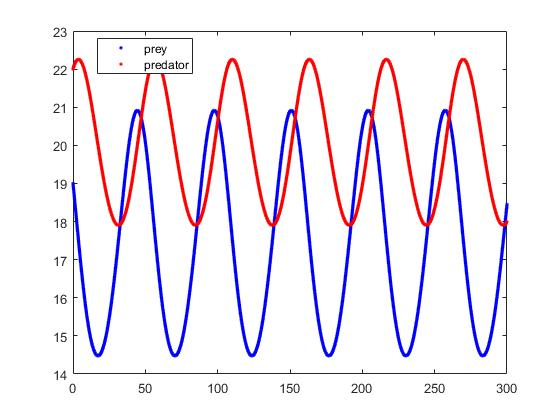
\includegraphics[width=\linewidth]{ex5.jpg}
			\caption{Evolution of the number of preys and predators.}
			\label{fig:ex5}
		\end{figure}

	
	\section*{Results}
	% comments to the results
	
	
	\section*{Outputs}
	
	
	
\end{document}



